% Aspectratio 16:9 should be used
% The theme is not suited for 4:3 aspectratio
\documentclass[aspectratio=169]{beamer}

\usepackage{mhchem}
\usepackage{tikz}
\usetikzlibrary{arrows.meta}
% Metadata of the presentation
\title{\ce{H3} as a model for open shell systems}
\subtitle{CIS with CUHF and UHF references}
\date[ISBT 2018]{Bachelor project}
\author[DB]{Ruben Van der Stichelen}

% Macro aimed at loading themes in different directories
\makeatletter
  \def\beamer@calltheme#1#2#3{%
    \def\beamer@themelist{#2}
    \@for\beamer@themename:=\beamer@themelist\do
    {\usepackage[{#1}]{\beamer@themelocation/#3\beamer@themename}}}

  \def\usefolder#1{
    \def\beamer@themelocation{#1}
  }
  \def\beamer@themelocation{}

% Load the UGent theme
\usefolder{theme}
\usetheme[language=en,faculty=we,usecolors]{ugent}
\useinnertheme{ugent}
\useoutertheme{ugent}
\usecolortheme{ugent}
\usefonttheme{ugent}

% Path to images
\graphicspath{{figures/}}

% Have this if you'd like section slides 
\AtBeginSection[]{
    \sectionframe
}

\begin{document}

% Have this if you'd like the presentation to start 
% with a large UGent logo
\logoframe

% I guess you always want a titleframe
\titleframe

% Start of the first section
\section{Introduction}

\begin{frame}
    \frametitle{The Hartree-Fock approximation}
The Schrödinger equation
    \begin{equation}
        \hat{H}\Psi = E\Psi
    \end{equation}
The Roothaan-Hall equation
\begin{equation}
    \mathbf{FC} = \epsilon \mathbf{SC}
\end{equation}
One constraint $\Longrightarrow$ energy minimum
    \begin{equation}
        \langle \psi + \delta\psi | \hat{H} | \psi + \delta\psi \rangle = E + \delta E^* + \delta E + \delta E^2 = E
    \end{equation}

\end{frame}

\begin{frame}
    \frametitle{Restricted Hartree-Fock}
    \begin{itemize}
        \item Electrons forced into pairs
        \item Higher energy
        \item Symmetry intact
    \end{itemize}
    \begin{minipage}[b]{0.6\linewidth}
        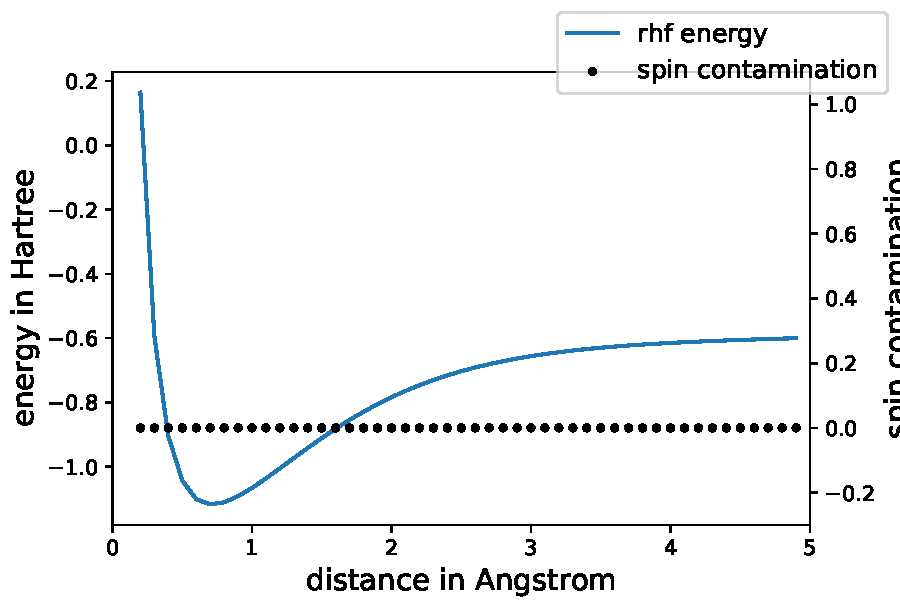
\includegraphics[width=\linewidth]{./figures/rhf.pdf}
    \end{minipage}

\end{frame}


\begin{frame}
    \frametitle{Unrestricted Hartree-Fock}
    \begin{itemize}
        \item No electron pairs
        \item Lower energy
        \item $\langle\hat{S}^2\rangle$ lost as quantum number
    \end{itemize}
    \begin{minipage}[b]{0.6\linewidth}
        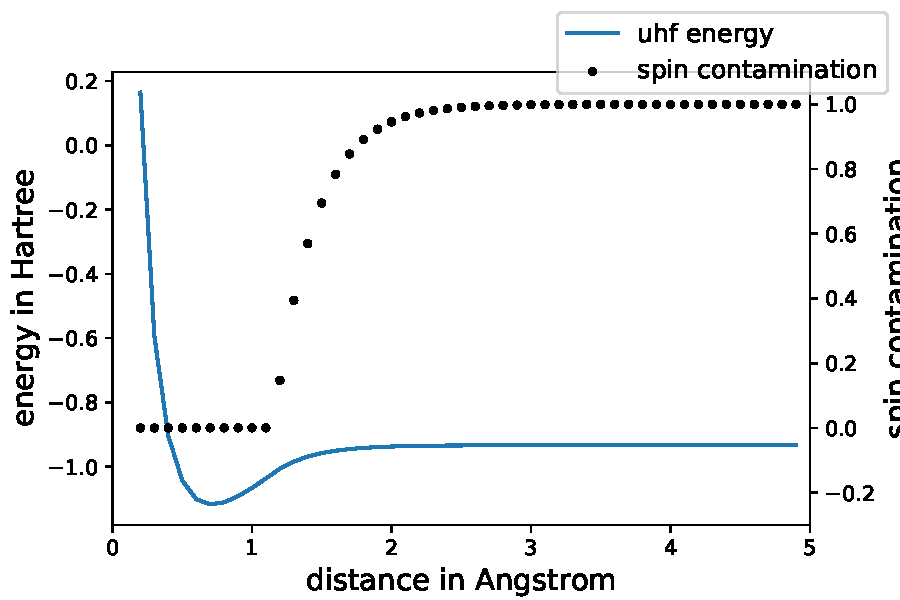
\includegraphics[width=\linewidth]{./figures/uhf.pdf}
    \end{minipage}
    \begin{minipage}[b]{0.35\linewidth}
        \begin{equation}
            \delta s = \langle \hat{S}^2 \rangle - S_z(S_z + 1)
        \end{equation}
    \end{minipage}
\end{frame}


\begin{frame}
    \frametitle{Löwdin's symmetry dillema}
    \begin{itemize}
        \item Low energy $\Longrightarrow$ loss of symmetry
        \item Keeping symmetry $\Longrightarrow$ high symmetry
        \item Do we always lose?
    \end{itemize}


\begin{itemize}
    \item Can we keep both symmetry and lower energies?
    \begin{itemize}
        \item ROHF
        \item CUHF
    \end{itemize}
\end{itemize}

\end{frame}

\section{Theory}

\begin{frame}
    \frametitle{Constrained unrestricted Hartree-Fock theory}
    \begin{equation}\label{eq:spincontfinal}
        \delta_s = 4\sum^{N_{cp}}_i n_i^2 - n_i
      \end{equation}
    \begin{equation}
        \tilde{F}^{\sigma} = F_{cs} \pm \Delta^{CUHF}
    \end{equation}
    where
    \begin{equation}
        \Delta^{CUHF} = \begin{cases}
            0, & \mbox{in the vc blocks} \\
            \Delta^{UHF}, & \mbox{anywhere else}
        \end{cases}
    \end{equation}
    $\Longrightarrow$ transformations needed
\end{frame}

\begin{frame}
    \begin{figure}
        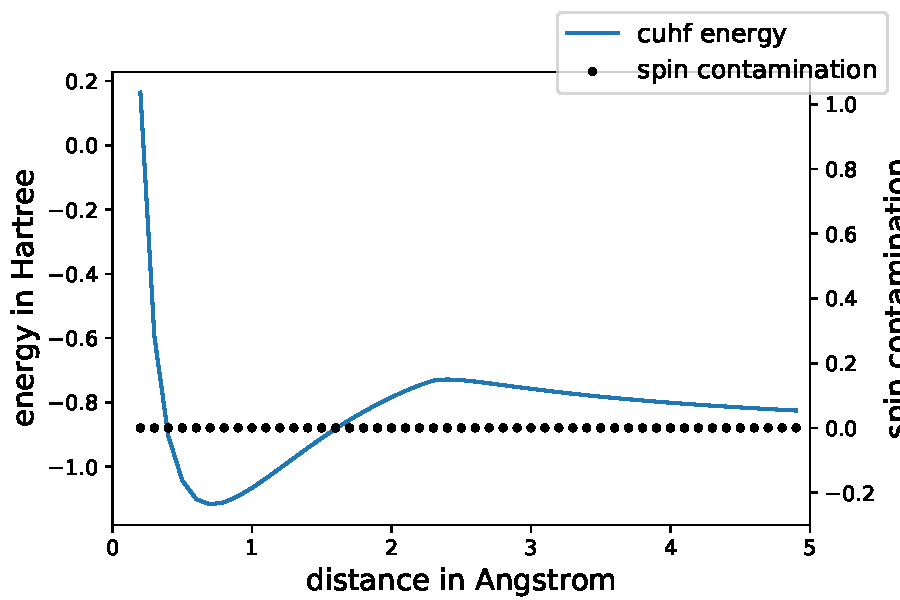
\includegraphics[width=0.6\linewidth]{./figures/cuhf_mix.pdf}
    \end{figure}
\end{frame}

\begin{frame}
    \frametitle{Configuration interaction} 
    \begin{equation}\label{eq:lincomb}
        |\Psi_0\rangle = c_0|\Phi_0\rangle + \sum_{ar}c_{r}^{a}|\Phi_r^a\rangle + \sum_{a<b,r<s}c_{rs}^{ab}|\Phi^{ab}_{rs} \rangle + \cdots
      \end{equation}
      Brillouin's theorem:
      \begin{equation}\label{eq:overlapsingle}
        \langle\Phi_0 |\hat{H}|\Phi_r^a\rangle = \langle a|h|r \rangle + \sum_b \langle ab||rb \rangle = \langle \chi_a |\hat{f}| \chi_r \rangle = F_{ra} = 0
      \end{equation}
      \begin{equation}\label{eq:matrixelement}
        \langle \Phi_r^a|\hat{H}|\Phi_s^b \rangle = E_0\delta_{rs}\delta_{ab} + F_{ab}\delta_{rs} - F_{rs}\delta_{ab} + \langle as || jb \rangle
      \end{equation}
\end{frame}


\section{results}

\begin{frame}
    \frametitle{Goals}
    \begin{enumerate}
        \item Excitation energy levels
        \item Differences/similarities between methods
        \begin{itemize}
            \item UHF
            \item CUHF
            \item ROHF
        \end{itemize}
        \item Spin contamination in the excited states
    \end{enumerate}

    

\end{frame}

\begin{frame}
    \frametitle{\ce{H3}}
    \begin{figure}
        \begin{minipage}[b]{0.45\linewidth}
            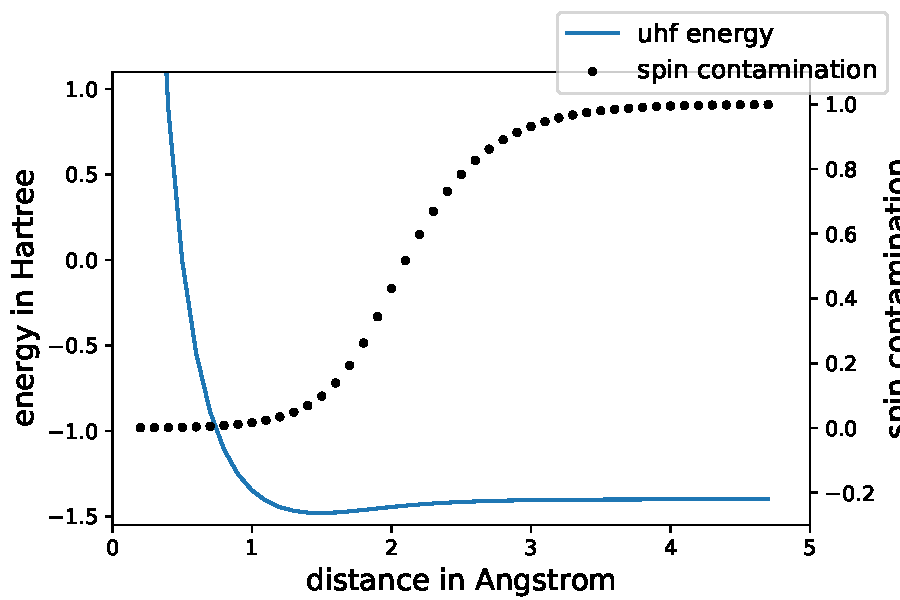
\includegraphics[width=\linewidth]{./figures/h3_uhf_sto-3g.pdf}
        \end{minipage}
        \begin{minipage}[b]{0.45\linewidth}
            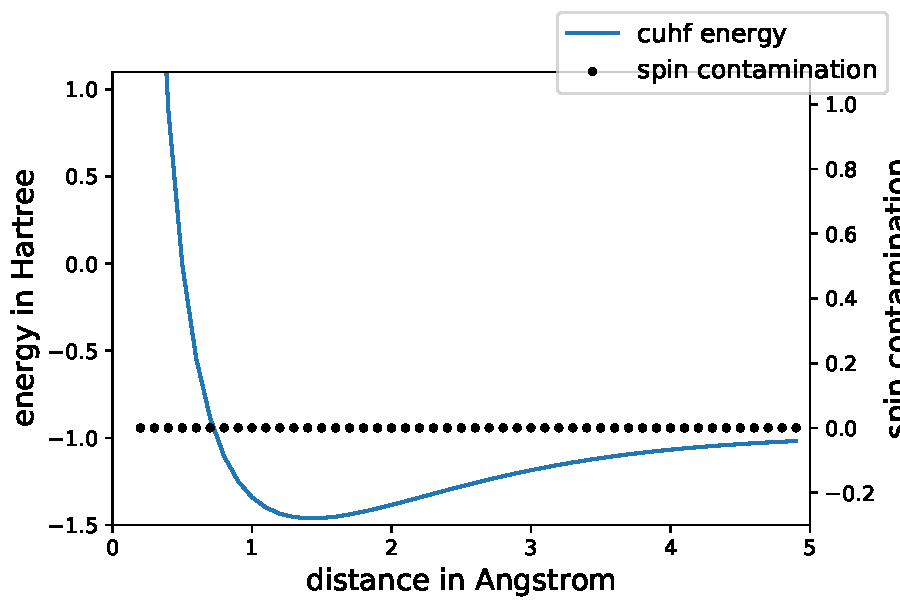
\includegraphics[width=\linewidth]{./figures/h3_cuhf.pdf}
        \end{minipage}
    \end{figure}

\end{frame}


\begin{frame}
    \frametitle{CUHF and UHF}
    \begin{minipage}[b]{0.6\linewidth}
        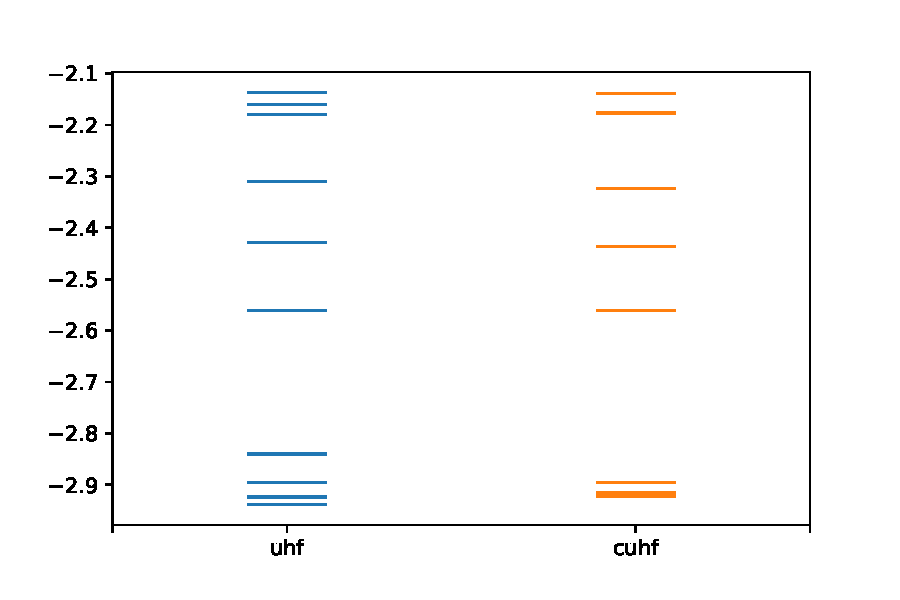
\includegraphics[width=\linewidth]{./figures/h3_cis.pdf}
    \end{minipage}
    \begin{minipage}[b]{0.3\linewidth}
        \begin{table}[h]
            \label{tab:excits}
            \begin{tabular}{l|l|l}
                 & UHF       & CUHF      \\
              \hline
              1  & -2.938139 & -2.922658 \\
              2  &  {\color{ugent-re}   \textbf{-2.923512}} & {\color{ugent-re}   \textbf{-2.915707}} \\
              3  & -2.896022 & {\color{ugent-re}   \textbf{-2.915707}} \\
              4  & -2.840079 & -2.895707 \\
              5  & -2.560947 & -2.560947 \\
              6  & -2.428072 & -2.436524 \\
              7  & -2.309793 & -2.323014 \\
              8  & -2.179570 & -2.176621 \\
              9  & -2.160308 & -2.176621 \\
              10 & -2.137036 & -2.139049
            \end{tabular}
          \end{table}
    \end{minipage}
    \begin{itemize}
        \item degeneracies
        \item lower energy states
    \end{itemize}
\end{frame}

\begin{frame}
    \frametitle{CUHF and ROHF}

\begin{minipage}[b]{0.35\linewidth}
    \begin{table}
        \label{tab:ROHF}
        \begin{tabular}{l|l}
            & energy    \\
          \hline
          1 & -2.915707 \\
          2 & -2.176621
        \end{tabular}
      \end{table}
\end{minipage}
\begin{minipage}[b]{0.6\linewidth}
    \begin{center}
    \includegraphics[width=0.8\linewidth]{./figures/H3_1_b_rohf.png}
    \includegraphics[width=0.8\linewidth]{./figures/H3_2_b_rohf.png}
    \end{center}
\end{minipage}
\end{frame}
\begin{frame}
    \frametitle{$\hat{S}^2$ expectation values}
    \begin{table}[h]
        \label{tab:spincon}
        \begin{tabular}{l|l|l}
            & UHF      & CUHF     \\
          \hline
          1 & 0.75     & 0.75     \\
          2 & 0.759614 & 0.752480 \\
          3 & 1.098750 & 1.148304 \\
          4 & 1.739963 & 1.750000 \\
          5 & 1.401673 & -1.34921
        \end{tabular}
      \end{table}
\end{frame}
\section{Conclusions and prospects}
\begin{frame}
    \frametitle{Conclusions and prospects}
    \begin{itemize}
        \item CUHF takes care of spin contamination in the ground state
        \item Things to look out for in CIS
        \begin{itemize}
            \item triplet excitations with lower energy (for some systems)
            \item spin contamination
        \end{itemize}
        \item Prospects
        \begin{itemize}
            \item triplet systems
            \item Higher order CI
            \item Other constraints $\Longrightarrow$ excited states?
        \end{itemize}
    \end{itemize}
    
\end{frame}

% End presentation with titleframe
\titleframe

\begin{frame}
    \begin{figure}[h]
        \begin{center}
          \begin{tikzpicture}
            \draw (-1.25, 0.5) -- (-0.75, 0.5);
            \draw (-1.25, 0) -- (-0.75, 0);
            \draw (-1.25, -0.5) -- (-0.75, -0.5);
            \draw [-{Straight Barb[left]}] (-1.1, -0.60) -- (-1.1, -0.20);
            \draw [-{Straight Barb[left]}] (-1.1, -0.10) -- (-1.1, 0.30);
            \draw [-{Straight Barb[left]}] (-0.9, -0.20) -- (-0.9, -0.60);
      
            \draw (1.25, 0.5) -- (0.75, 0.5);
            \draw (1.25, 0) -- (0.75, 0);
            \draw (1.25, -0.5) -- (0.75, -0.5);
            \draw [-{Straight Barb[left]}] (0.9, -0.60) -- (0.9, -0.20);
            \draw [-{Straight Barb[left]}] (1.1, 0.30) -- (1.1, -0.10);
            \draw [-{Straight Barb[left]}] (1.1, -0.20) -- (1.1, -0.60);
          \end{tikzpicture}
        \end{center}
      \end{figure}
      $\Longrightarrow$ The ground state is degenerate
    \begin{table}[h]
        \label{tab:excits_no_triplets}
        \begin{tabular}{l|l|l}
            & UHF       & CUHF      \\
          \hline
          1 & {\color{ugent-re}   \textbf{-2.923512}} & {\color{ugent-re}   \textbf{-2.915707}} \\
          2 & -2.840101 & -2.895707 \\
          3 & -2.428086 & -2.436524 \\
          4 & -2.160319 & -2.176620 \\
          5 & -2.137039 & -2.139049
        \end{tabular}
      \end{table}
\end{frame}

\end{document}
